\documentclass[11pt]{article}
\usepackage[letterpaper,margin=0.78in]{geometry}
\usepackage{amsmath,amssymb,amsthm,mathtools}
\usepackage{graphicx,microtype,enumitem,booktabs,xcolor}
\usepackage[colorlinks=true,linkcolor=blue!45!black,urlcolor=blue!55!black,citecolor=blue!45!black]{hyperref}
\setlist{nosep,leftmargin=1.6em}
\newtheorem{theorem}{Theorem}
\newcommand{\vp}{\varphi}
\newcommand{\meet}{\mathbin{\wedge}}
\definecolor{answer}{RGB}{26,105,73}
\pagestyle{plain}

\title{The quotient questions for \(f\)-algebras\\
\large A literature resolution and elementary verification of Questions 8.3 in arXiv:2005.00902}
\author{Automated mathematical discovery run \texttt{fa\_banach\_001}, lane 9}
\date{17 August 2026}

\begin{document}
\maketitle

\begin{center}
\fcolorbox{answer}{answer!7}{\parbox{0.91\linewidth}{
\textbf{Disposition: literature already answered.}
All three questions have affirmative answers.  The later paper
Mu\~noz--Lahoz--Tradacete, arXiv:2511.13299, explicitly records that
\(f\)-algebras form an equational class, citing Birkhoff's \emph{Lattice
Theory}, Theorem VII.8, and notes that free \(f\)-algebras have been known
since 1956.  The proof below independently verifies the claim and displays
two explicit defining identities, but is not asserted to be new.
}}
\end{center}

\section*{Source question and transcription}
Let \(A\) be an \(f\)-algebra, let \(B\) be a vector lattice algebra, and
let \(\vp:A\to B\) be a surjective vector lattice algebra homomorphism.
Questions 8.3 ask:
\begin{enumerate}
\item Must \(B\) be an \(f\)-algebra?
\item Is the answer still affirmative when \(A\) is unital?
\item Is the answer still affirmative when \(A\) is unital with positive
identity?
\end{enumerate}
The source observes that affirmative answers make the corresponding three
classes equational and yield free objects over nonempty sets.

\section*{Definitions}
A vector lattice algebra is an associative real algebra which is also a
vector lattice and whose positive cone is closed under multiplication.  It is
an \(f\)-algebra when, for \(x,y\in A\) and \(z\in A_+\),
\[
 x\meet y=0 \quad\Longrightarrow\quad
 (xz)\meet y=(zx)\meet y=0.
\]
A vector lattice algebra homomorphism preserves the linear, lattice, and
algebra operations.  The kernel of a surjective such homomorphism is a
two-sided algebra ideal and an order ideal.

\section*{Idea / proof intuition}
There are two short routes.  First, replace arbitrary positive elements
\(x,y\) by the disjoint remainders \(x-x\meet y\) and \(y-x\meet y\).  This
turns the conditional \(f\)-algebra axiom into two unconditional identities.
Second, in a quotient write \(x=u+x_0\), \(y=u+y_0\), where
\(u=x\meet y\) lies in the kernel and \(x_0\perp y_0\).  After multiplying,
the only term not visibly controlled by the kernel vanishes by the
\(f\)-algebra property.

\clearpage
\section*{Original source image}
\begin{center}

\includegraphics[width=0.96\textwidth,height=0.88\textheight,keepaspectratio]{source_question_crop.png}
\end{center}
\smallskip
\noindent\footnotesize Source: de Jeu, arXiv:2005.00902, PDF p.~35,
Questions 8.3.  This is a direct crop from \texttt{source\_paper.pdf}.

\clearpage
\section*{Later literature answer}
The later paper \emph{The free Banach \(f\)-algebra generated by a Banach
space} states that the existence of free \(f\)-algebras is long known and
follows from the fact that \(f\)-algebras form an equational class.  It cites
Keimel's 1995 survey, Section 5.2, and Birkhoff's 1961 \emph{Lattice Theory},
Theorem VII.8.  Its introduction also attributes the foundational theory to
Birkhoff--Pierce (1956).

\begin{center}
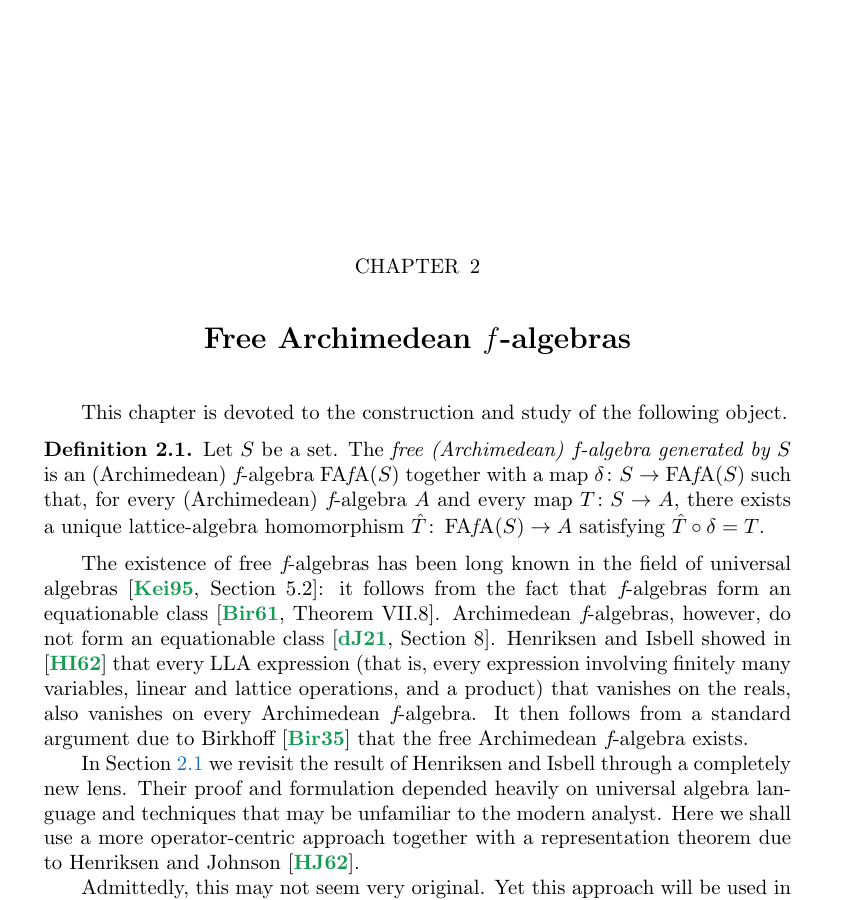
\includegraphics[width=0.94\textwidth,height=0.72\textheight,keepaspectratio]{literature_answer_crop.png}
\end{center}
\noindent\footnotesize Source: Mu\~noz--Lahoz--Tradacete,
arXiv:2511.13299, PDF p.~23 (printed p.~11).  This is a direct crop from
the supporting PDF stored with this packet.

\clearpage
\section*{Elementary verification}
For \(a,b\) in a vector lattice put
\[
 r(a,b)=a^+-(a^+\meet b^+),\qquad
 s(a,b)=b^+-(a^+\meet b^+).
\]
Then \(r(a,b),s(a,b)\geq0\) and \(r(a,b)\meet s(a,b)=0\).

\begin{theorem}[Explicit equations and quotient stability]
Among vector lattice algebras, the \(f\)-algebras are exactly those satisfying
the two identities
\begin{align*}
 \bigl(r(a,b)c^+\bigr)\meet s(a,b)&=0,\\
 \bigl(c^+r(a,b)\bigr)\meet s(a,b)&=0
\end{align*}
for all \(a,b,c\).  Consequently every surjective vector lattice algebra
homomorphic image of an \(f\)-algebra is an \(f\)-algebra.  The same holds in
the unital and positive-unital signatures.
\end{theorem}

\begin{proof}
If \(A\) is an \(f\)-algebra, the displayed identities follow because
\(r(a,b)\) and \(s(a,b)\) are positive and disjoint, while \(c^+\geq0\).
Conversely, suppose the identities hold and \(x\meet y=0\), \(z\geq0\).
Then \(x,y\geq0\), and substituting \((a,b,c)=(x,y,z)\) gives
\(r=x\), \(s=y\), hence \((xz)\meet y=(zx)\meet y=0\).  Thus the identities
are equivalent to the \(f\)-algebra axiom.

For a direct quotient check, let \(q:A\to B\) be surjective and
\(I=\ker q\).  Given \(\bar x,\bar y,\bar z\geq0\) in \(B\) with
\(\bar x\meet\bar y=0\), choose positive lifts \(x,y,z\).  Set
\(u=x\meet y\in I\), \(x_0=x-u\), and \(y_0=y-u\).  Then
\(x_0\meet y_0=0\), so \((x_0z)\meet y_0=0\).  For positive elements of
any vector lattice,
\[
 (a+b)\meet(c+d)
 \leq(a\meet c)+(a\meet d)+(b\meet c)+(b\meet d),
\]
which follows twice from the Riesz decomposition property.  Therefore
\begin{align*}
 (xz)\meet y
 &= (uz+x_0z)\meet(u+y_0)\\
 &\leq (uz\meet u)+(uz\meet y_0)+(x_0z\meet u)
       +(x_0z\meet y_0)\\
 &\leq 2u+uz\in I.
\end{align*}
As \(I\) is an order ideal, \((xz)\meet y\in I\), and hence
\((\bar x\bar z)\meet\bar y=0\).  Replacing right multiplication by left
multiplication gives \((\bar z\bar x)\meet\bar y=0\).  Thus \(B\) is an
\(f\)-algebra.  If \(A\) is unital, surjectivity sends its identity to the
identity of \(B\); positivity of the identity is likewise preserved.
\end{proof}

\clearpage
\section*{Consequences, verification, and scope}
\begin{itemize}
\item Questions 8.3(1)--(3) all have affirmative answers.
\item The two displayed identities give an explicit equational
axiomatization after adjoining the standard vector-lattice-algebra identities.
The unital and positive-unital subclasses add the usual unit identities.
\item Birkhoff's variety theorem therefore yields free \(f\)-algebras, free
unital \(f\)-algebras, and free positive-unital \(f\)-algebras over nonempty
sets.
\item The proof is algebraic: it uses neither Archimedeanness nor a norm, and
it treats noncommutative multiplication by retaining both left and right
identities.
\end{itemize}

\paragraph{Verification.}
The positivity of lifts follows from surjectivity and
\(q(a^+)=q(a)^+\).  The kernel is both an order ideal and a two-sided algebra
ideal.  The four-term meet inequality is valid in arbitrary (including
non-Archimedean) vector lattices by Riesz decomposition.  These checks remove
the three main hidden failure modes in the quotient argument.

\paragraph{Novelty and limitations.}
This packet is a literature-resolution record, not a novelty claim.  The later
arXiv paper explicitly identifies the result as classical and gives the
primary classical citations.  No attempt was made here to settle the distinct
Questions 8.4 asking whether particular free \emph{vector lattice algebras}
are themselves \(f\)-algebras or Archimedean.

\paragraph{Human review.}
Pending.  Recommended check: compare the signature used in Birkhoff,
Theorem VII.8, with the associative real vector lattice algebra signature of
the source.  The self-contained proof above independently covers exactly the
source signature.

\section*{References}
\begin{enumerate}[label={[\arabic*]}]
\item M. de Jeu, \emph{Free vector lattices and free vector lattice
algebras}, arXiv:2005.00902 (2020/2021), Section 8.
\item D. Mu\~noz--Lahoz and P. Tradacete, \emph{The free Banach
\(f\)-algebra generated by a Banach space}, arXiv:2511.13299 (2025/2026),
Chapter 2.
\item G. Birkhoff, \emph{Lattice Theory}, revised ed., AMS Colloquium
Publications XXV, 1961, Theorem VII.8.
\item G. Birkhoff and R. S. Pierce, \emph{Lattice-ordered rings}, An. Acad.
Brasil. Ci. 28 (1956), 41--69.
\item K. Keimel, \emph{Some trends in lattice-ordered groups and rings},
1995, Section 5.2.
\end{enumerate}

\end{document}
